\documentclass{article}

\usepackage{fancyhdr}
\usepackage{graphicx}
\usepackage{float}
\usepackage{geometry}
\geometry{margin=1in}
\setlength{\headheight}{49.4pt}
\pagestyle{fancy}
\fancyhf{}
\rhead{
    \centering
  \begin{tabular*}{\textwidth}{@{\extracolsep{\fill}}ccc}
    \small University of Florida & \textbf{\small EEL3111C - Circuits} & \small Rottenberg, Cole Harrison\\
    \small Electrical \& Computer Engineering Dept. & \small Lab 10: Final Project & \small Class \#: 20931 \\
    \small Page \thepage & \small Revision: 0 & \small \today \\
  \end{tabular*}
}

\begin{document}
% I need a bold horizontal line

\begin{center}
    \hrule
    \vspace{0.2cm}
    \textbf{\large REQUIREMENTS NOT MET}
    \vspace{0.2cm}
    \hrule
\end{center}
% Bullet points on what was not met
\begin{itemize}
    \item \textbf{Requirement 1:} The requirement was not met because of this reason.
    \item \textbf{Requirement 2:} The requirement was not met because of this reason.
    \item \textbf{Requirement 3:} The requirement was not met because of this reason.
\end{itemize}

\begin{center}
    \hrule
    \vspace{0.2cm}
    \textbf{\large PROBLEMS ENCOUNTERED}
    \vspace{0.2cm}
    \hrule
\end{center}
% More Bullet points with filler text
\begin{itemize}
    \item \textbf{Problem 1:} The problem was encountered because of this reason.
    \item \textbf{Problem 2:} The problem was encountered because of this reason.
    \item \textbf{Problem 3:} The problem was encountered because of this reason.
\end{itemize}

\begin{center}
    \hrule
    \vspace{0.2cm}
    \textbf{\large INTRODUCTION}
    \vspace{0.2cm}
    \hrule
\end{center}

Now we start our introduction to our write up
For your write up, write a brief introduction to what you are doing in the in lab. two to four sentences. 
Omit this section for the prelab.


\begin{center}
    \hrule
    \vspace{0.2cm}
    \textbf{\large DISCUSSION}
    % A horizontal line here
    \vspace{0.2cm}
    \hrule
\end{center}

\textbf{10.4 Pre-Lab Requirements:} 

Image of the spice schematic and a plot of the input and all subsequent out-
puts (outputs of each individual stage) for a transient simulation for Jingle19
submitted to Canvas. Include the plot of the output and a circuit schematic,
nothing else. The schematic and plot should be appropriately labeled. Images
that are unclear or vague will receive little to no points. Your plot must include
the following in different plot planes: input voltage, output of the high pass
filter, output of the variable gain amplifier, output of the buffer stage (at least
one), and the current of both LEDs. The gain doesn’t need to be high enough
to induce clipping in order to show that both LEDs turn on but the first LED
should turn on.

\begin{itemize}
    \item Stage 1: Active High Pass Filter
    \begin{figure}[H]
        \centering
        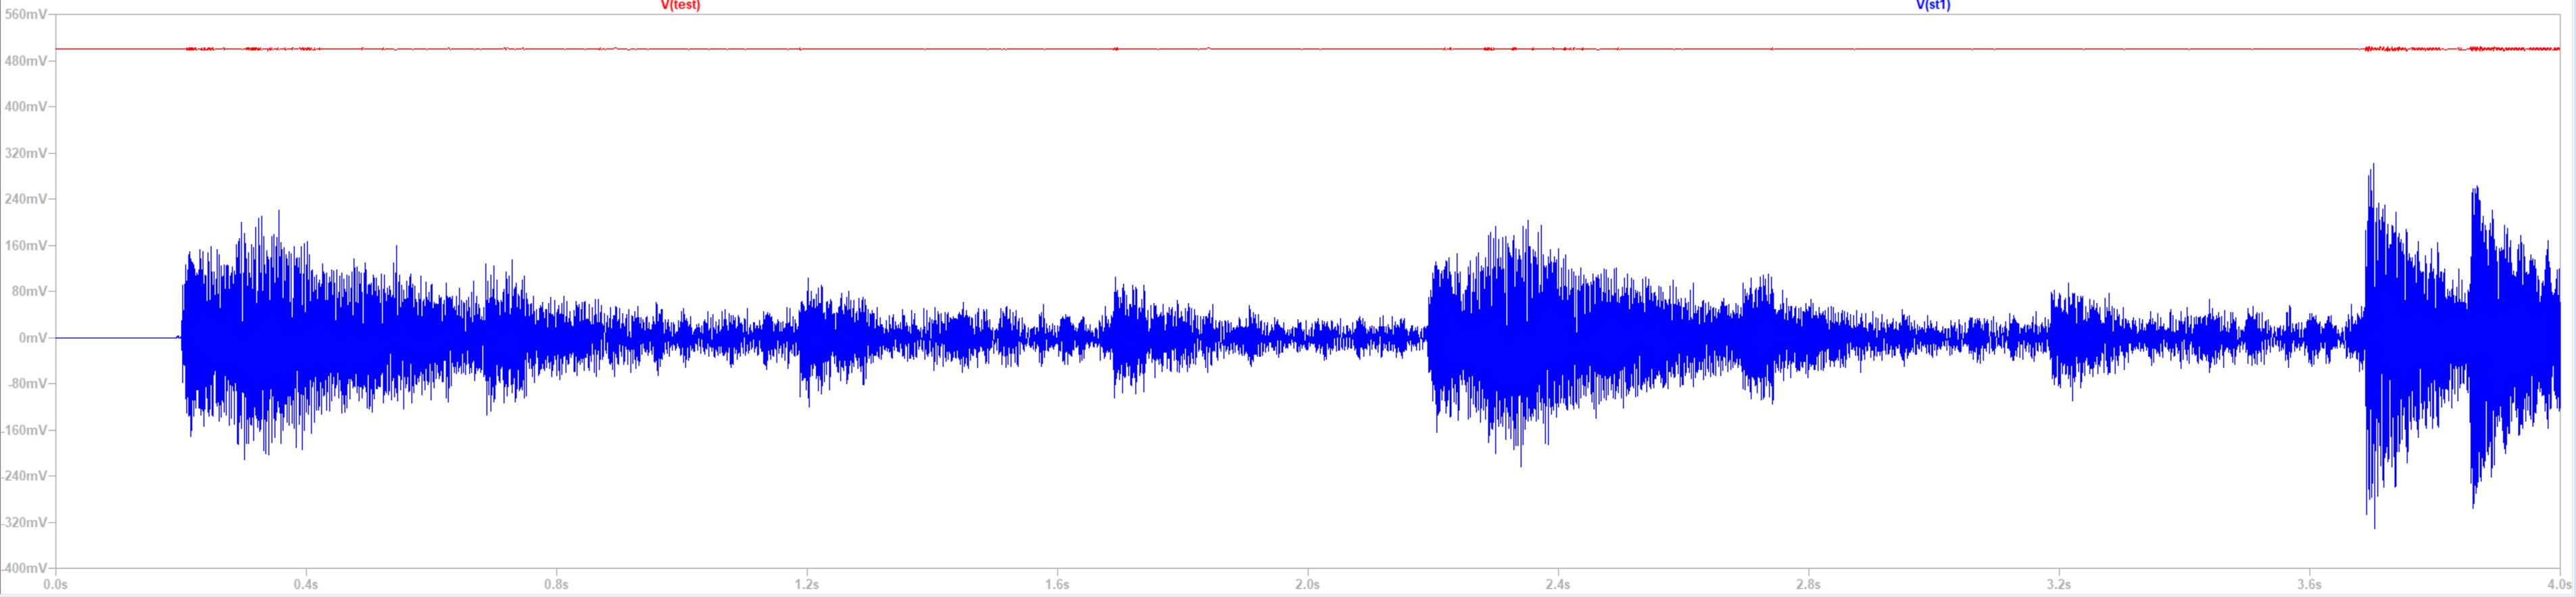
\includegraphics[width=1\textwidth]{activehighplot.png}
        \caption{Active High Pass with a Gain of 10}
    \end{figure}
    \item Stage 2: Active High Pass Filter
    \begin{figure}[H]
        \centering
        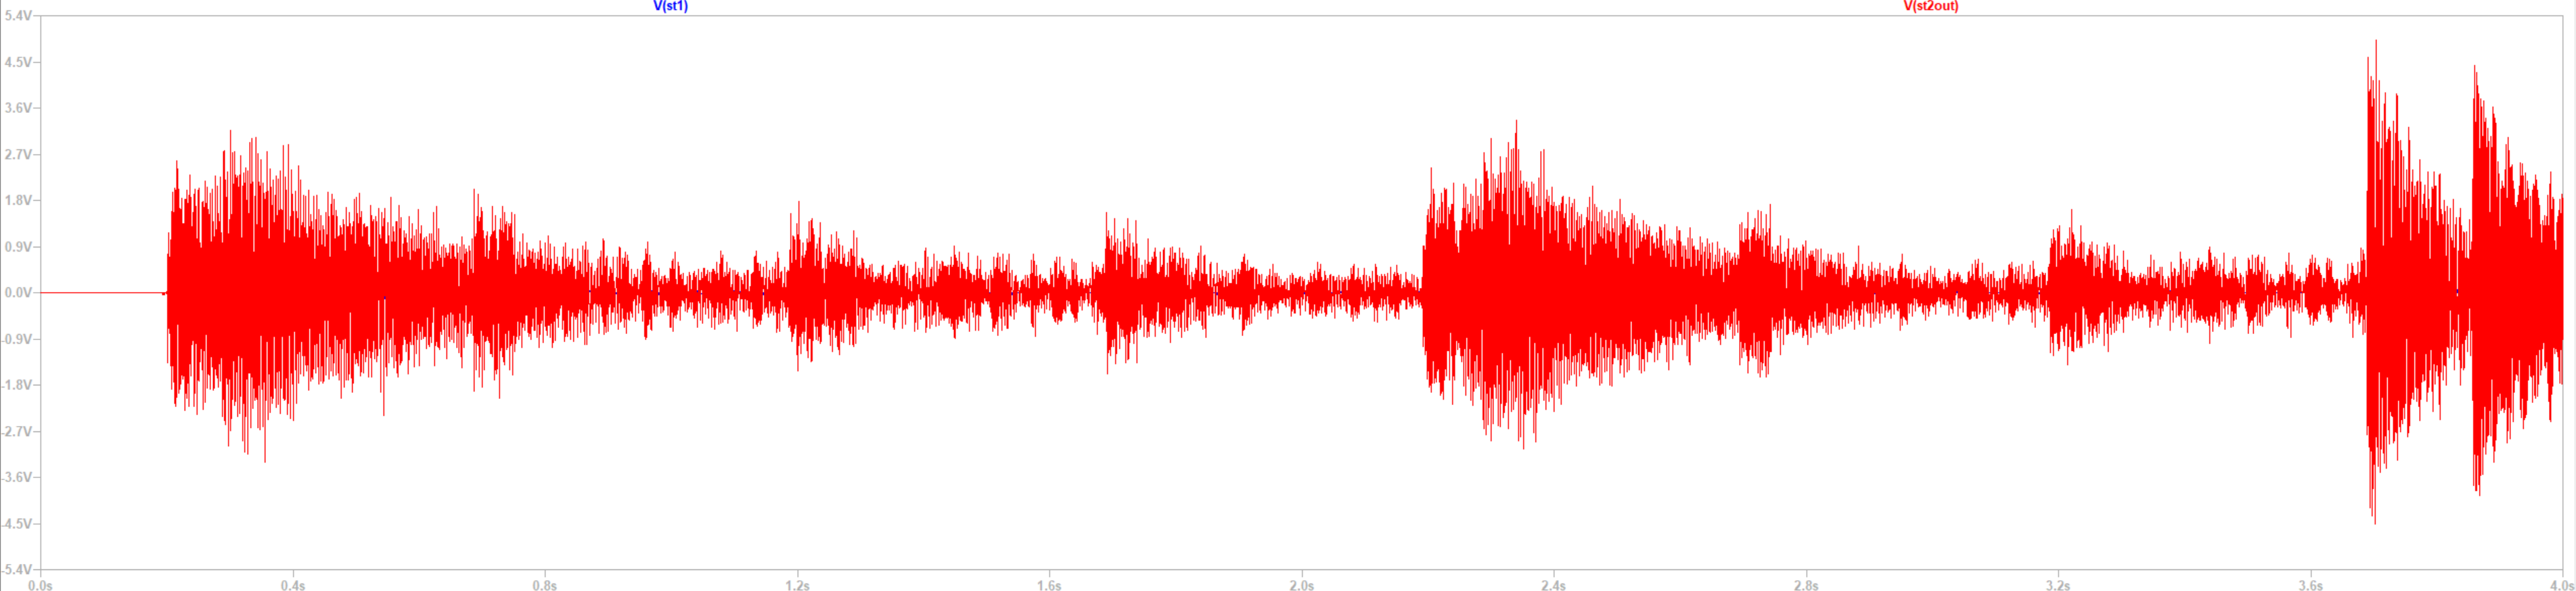
\includegraphics[width=1\textwidth]{gainstage.png}
        \caption{Inverting Amplifier with a Gain of 15}
    \end{figure}
    \item Stage 3: Comparator Stage
    \begin{figure}[H]
        \centering
        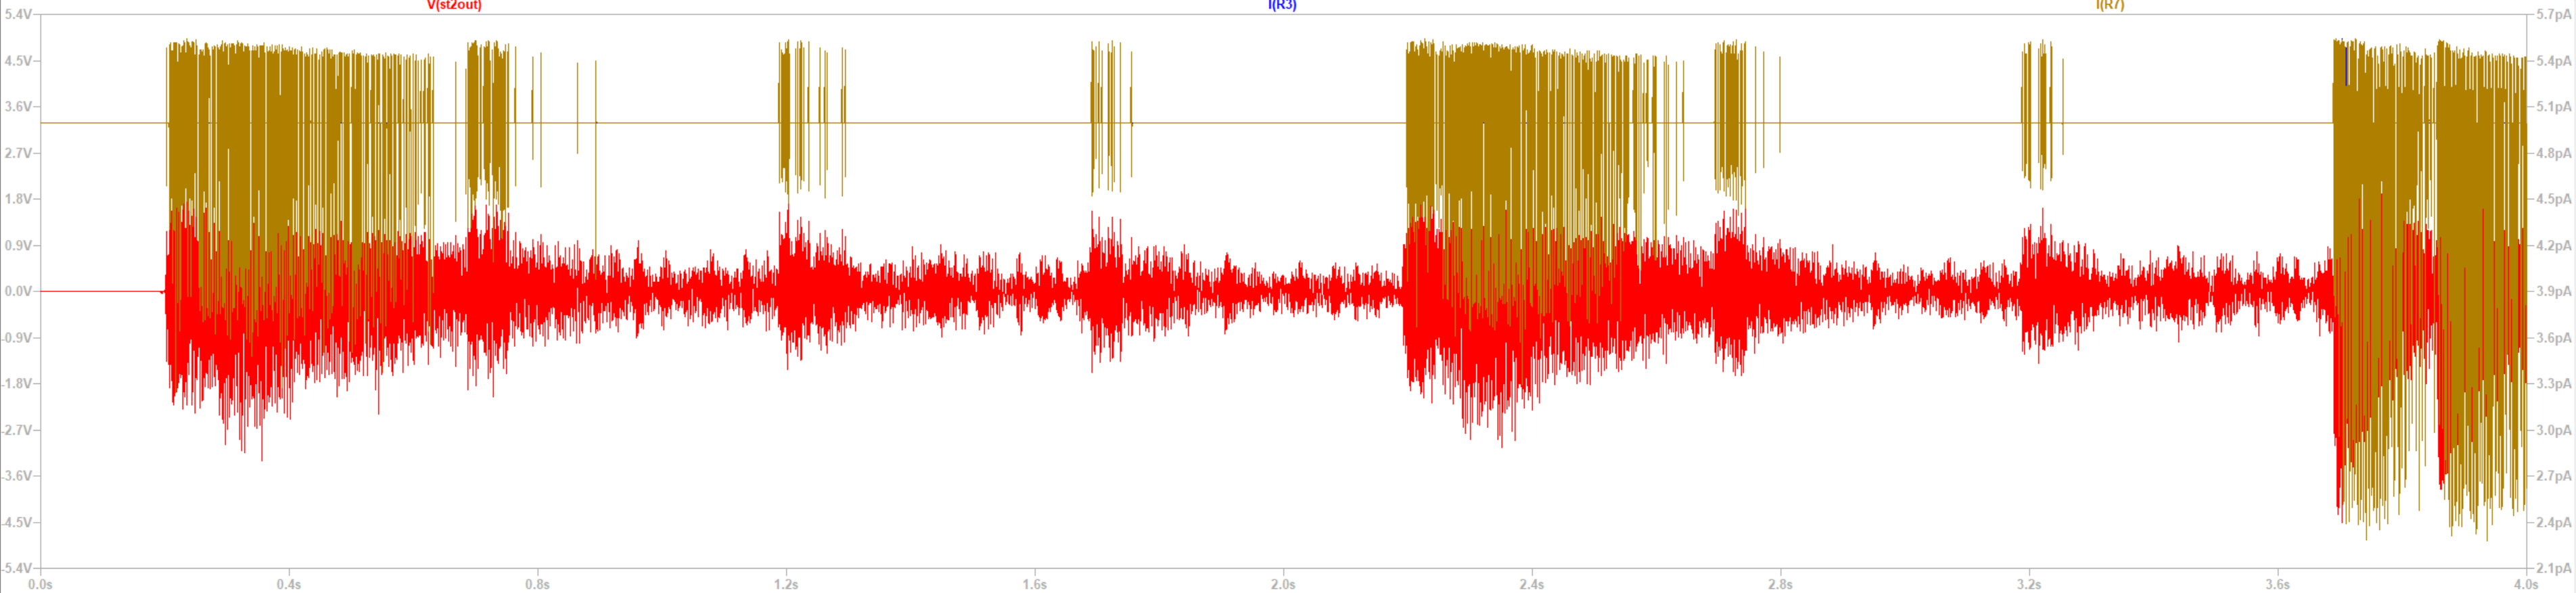
\includegraphics[width=1\textwidth]{compstage.png}
        \caption{Comparator measuring current through the LED}
    \end{figure}
    \item Stage 4: Buffer Stage 
    \begin{figure}[H]
        \centering
        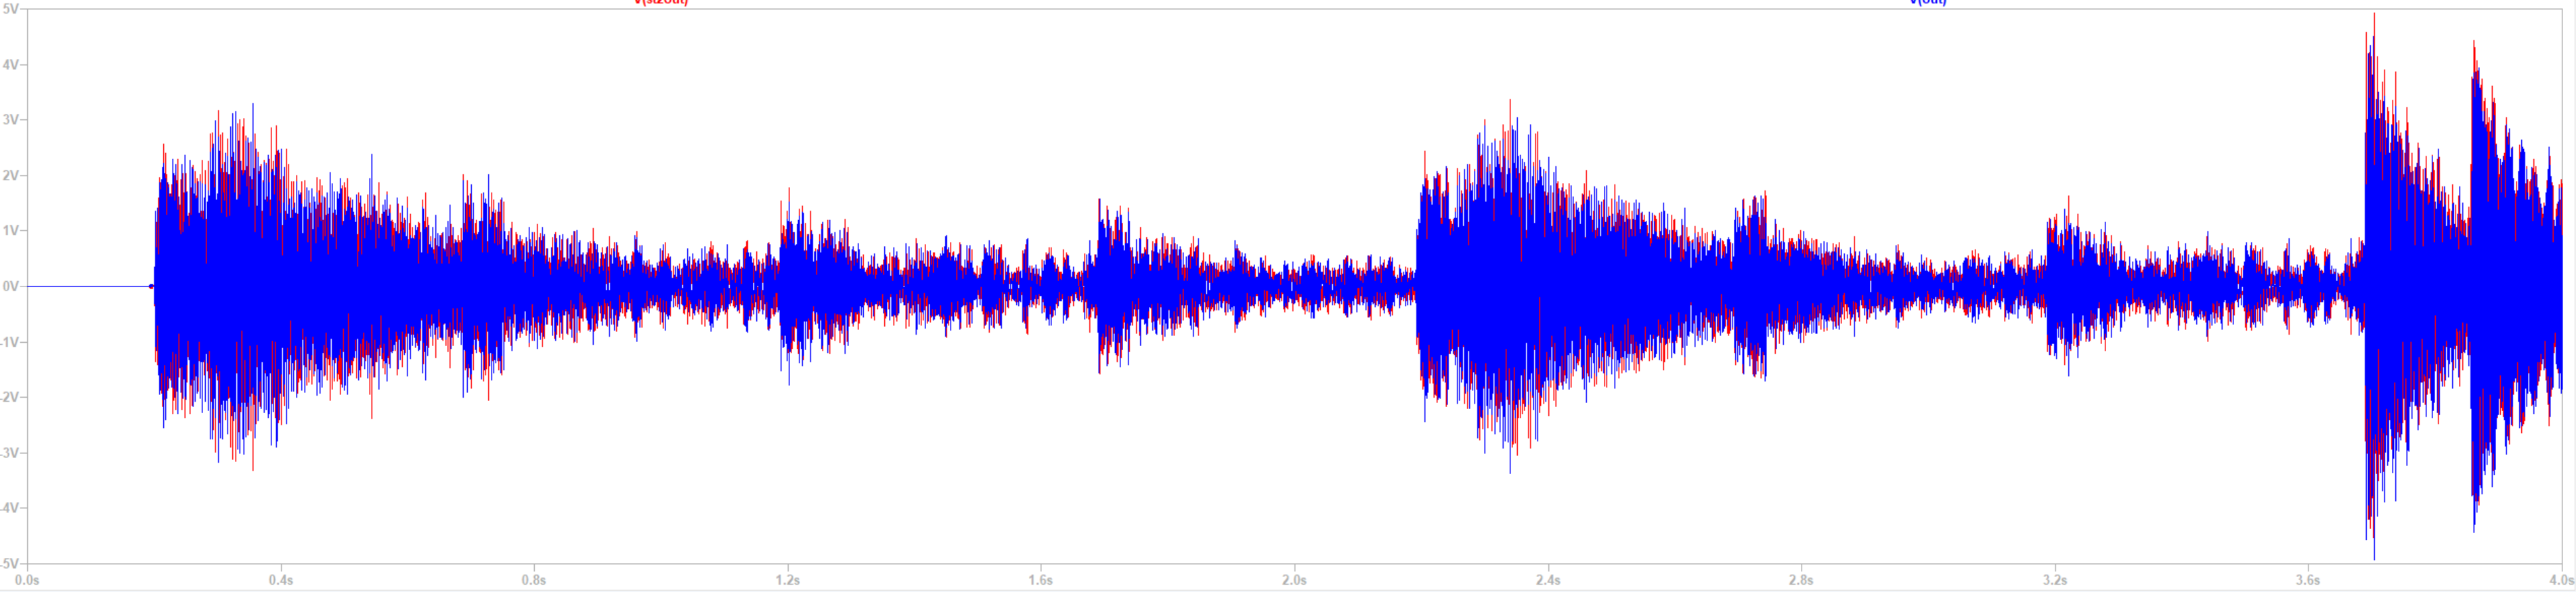
\includegraphics[width=1\textwidth]{buffstage.png}
        \caption{Voltage Following Buffer Stage}
    \end{figure}
    \item Circuit Schematic
    \begin{figure}[H]
        \centering
        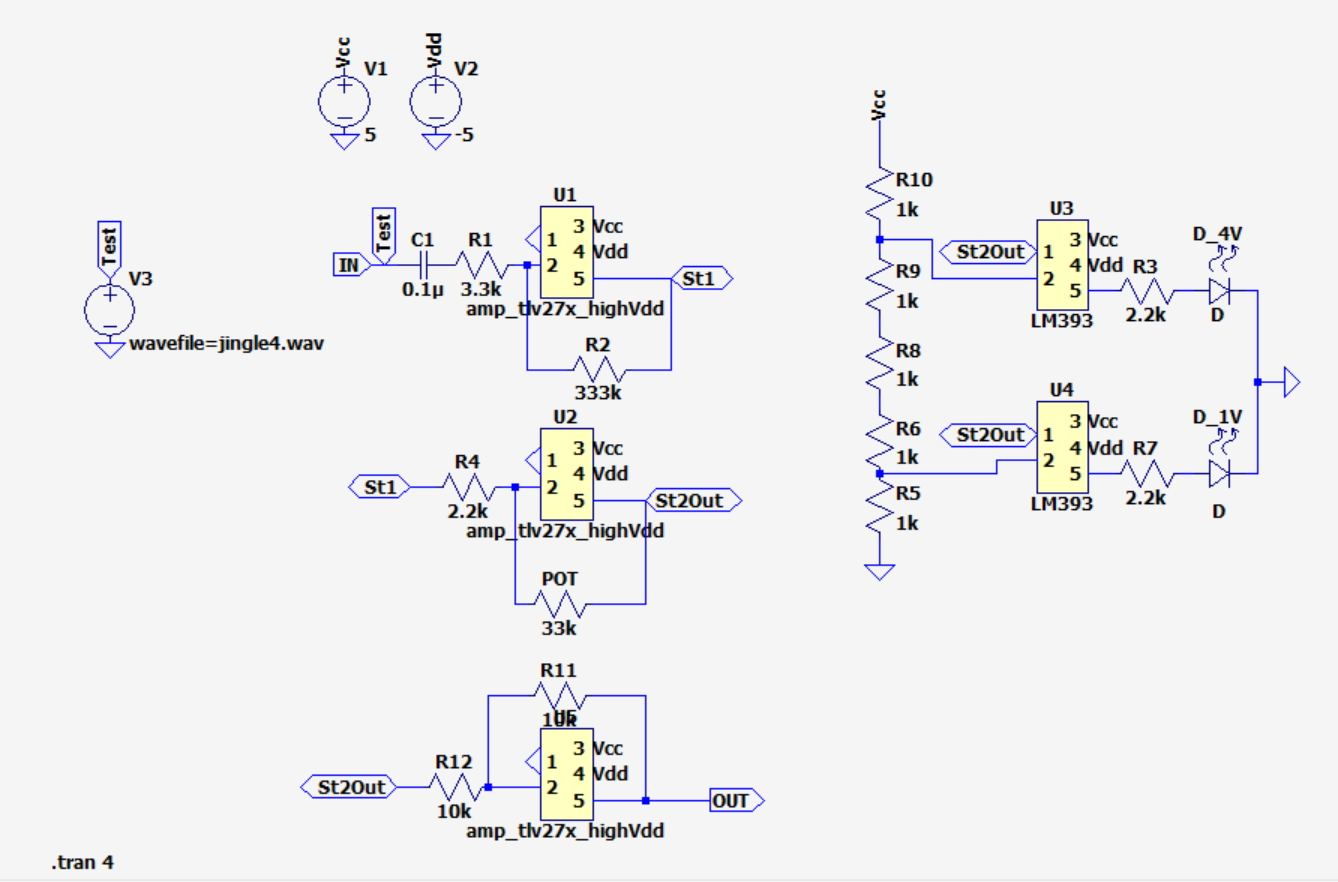
\includegraphics[width=1\textwidth]{circuitdiagram.png}
        \caption{Full Schematic of the Circuit and each stage}
    \end{figure}
\end{itemize}

\begin{center}
    \hrule
    \vspace{0.2cm}
    \textbf{\large CONCLUSION}
    % A horizontal line here
    \vspace{0.2cm}
    \hrule
\end{center}

This is where I start to answer the questions in the lab. We only need to do this for the write up.

\end{document}